\section{Methods}
\label{sec:methods}
\subsection{Source Sequences and Dataset Tasks}
\label{sec:benchmark_formulation}
GaitEval evaluates dataset-specified label prediction from pose-derived evidence. The six datasets and their evaluation partitions are listed in Table~\ref{tab:method_datasets}. GMFCS contains children with cerebral palsy~\cite{palisano1997gmfcs}; PARKINSONISM and CARE-PD concern Parkinson's disease with different severity or gait-item targets~\cite{deng2024parkinsonism,adeli2025carepd}. ATAXIA contains healthy volunteers imitating ataxic gait~\cite{khalil2023dataset}, and PATHOGAIT contains healthy volunteers simulating six gait patterns~\cite{jun2020pathological}. ASD-Kinect defines an autism-versus-typical task~\cite{aljubouri2021asd}; its source reports some movements simulated by others without identifying the affected sequences. These resources are therefore not six interchangeable clinical cohorts.

\begin{table*}[t]
\centering\small
\caption{\textbf{Six benchmark datasets for the seven-condition evaluation (source-reported subject-disjoint partitions).} Counts are eligible train/test clips and test participants, not full-source cohort sizes. All six datasets have summary and z-feature zero-shot, evidence/order controls, summary-SFT, and matched LR/SVM.}
\label{tab:method_datasets}
\begin{tabular*}{\textwidth}{@{\extracolsep{\fill}}lllrr@{}}\toprule
Dataset & Population & Task & Train / test & Test subjects\\\midrule
ASD-Kinect & ASD / typical; provenance caveat & Binary & 70 / 20 & 20\\
ATAXIA & Healthy, imitated gait & Binary & 28 / 8 & 4\\
CARE-PD & Multi-site Parkinson's cohort & UPDRS gait 0--3 & 1901 / 665 & 24\\
GMFCS & Cerebral-palsy cohort & Four-level ordinal & 914 / 255 & 149\\
PARKINSONISM & Parkinson's cohort & Binary severity & 83 / 29 & 5\\
PATHOGAIT & Healthy, simulated gait & Six patterns & 5040 / 1440 & 2\\\bottomrule
\end{tabular*}
\end{table*}

A source sequence is $X_i\in\mathbb{R}^{T_i\times J_d\times C_d}$, with dataset-specific joints and coordinate channels. Native 2D/3D representations follow established pose formats~\cite{cao2017openpose,ionescu2014human36m}. GaitEval applies one evaluation protocol: select task-eligible participant partitions; derive a label-redacted input view; run the declared model and evidence condition; fit supervised transformations on training data only; and score predictions against the complete task label set. Each experiment records its model, input construction, test IDs, and parser settings. The coordinate-input experiments use a 124-frame source tensor, with padding masked during feature computation; normalized-coordinate prompts sample 32 frames and 12 common joints. Feature and summary runs aggregate the valid trajectories in their recorded input construction.

All six datasets enter the seven-condition Qwen2.5-7B evaluation on the test sets in Table~\ref{tab:method_datasets}. Additional model, coordinate, few-shot, and feature-SFT experiments use the eligible records listed in the supplemental evaluation-record inventory; their test counts are also stated with the results. The GMFCS split-repair check uses 866 test clips from 166 participants; the seven-condition comparison uses 255 clips from 149 participants. Within an experiment, comparisons use matched test records; comparisons across different test populations are descriptive. Participant separation in the 866-clip experiment is independently verified. The seven-condition partitions are reported as subject-disjoint by the source metadata, but complete training manifests remain unavailable for an independent check. Section~\ref{sec:review_checks} documents the repair.

\subsection{Controlled Input Views}
\label{sec:input_views}
Each run exposes one view. Four input-view families are defined: raw coordinates, normalized coordinates, deterministic motion summaries, and named biomechanical features. A train-statistics z-scored encoding is a scaling control within the feature family, not a fifth modality. Coordinate prompting is a subset experiment; it is not claimed to have common six-dataset coverage.

Features describe motion range, bilateral asymmetry, trunk/pelvis variability, trajectory variance, and jerk-based smoothness~\cite{winter2009biomechanics,schwartz2008gdi}. Unsupported joints are omitted consistently from the LLM and matched linear inputs. These are pose-coordinate descriptors, not calibrated physical stride lengths or forces. The jerk descriptor uses third finite differences per frame and is not asserted to have SI jerk units. For feature $f$, scaling is $z=(f-\mu_{\rm tr})/\sigma_{\rm tr}$, using training statistics only; constant and missing-column handling is specified in the supplement.

Motion summaries are generated by a deterministic, label-independent template from the numerical measurements, not by annotators, dataset metadata, or another LLM. They preserve numbers and fixed qualitative descriptors. Capture-quality variables, including valid-frame fraction, are excluded from the seven shared feature/summary conditions. Model-visible inputs exclude answer-revealing labels, dataset names, participant IDs, demographics, and clinical metadata; candidate labels remain because they define the task. Figure~\ref{fig:method_detail} distinguishes these transformations.

\begin{figure}[t]
\centering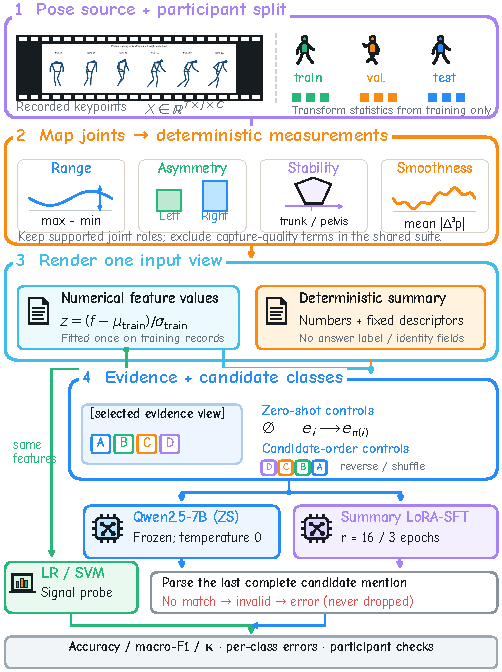
\includegraphics[width=\columnwidth]{figures/methods.pdf}
\caption{\textbf{Pose-to-label evaluation.} The shared six-dataset workflow links training-only transformations to zero-shot controls, summary-SFT, and matched linear references. Recorded GMFCS keyframes illustrate the source; measurement glyphs are schematic. Invalid outputs remain errors. Optional probes follow the supplemental coverage.}
\label{fig:method_detail}
\end{figure}

\subsection{Models, Adaptation, and Evidence Controls}
\label{sec:evaluation_settings}
The five-family motion-summary axis evaluates Llama-3.3-70B, Qwen2.5-72B, and Gemma-3-27B~\cite{grattafiori2024llama3,qwen2024qwen25,gemma2025gemma3}, together with GLM-4-32B and DeepSeek-R1-Distill-Qwen-32B~\cite{glm2024chatglm,guo2025deepseekr1}. The shared six-dataset axis fixes Qwen2.5-7B-Instruct. The test counts for the five-model comparison are 20, 1,647, 665, 866, 120, and 2,181 clips in dataset order; the corresponding Qwen-7B shared-condition counts are in Table~\ref{tab:method_datasets}. Full settings and coverage are in the supplement.

All six datasets use seven common conditions: summary zero-shot; z-feature zero-shot; no evidence; shuffled evidence; reversed and shuffled candidate order; and summary LoRA-SFT. Shuffled evidence deranges summaries across test records while preserving candidate labels. Candidate-order controls preserve evidence and change only label presentation. Decoding is deterministic. The parser chooses the last complete, boundary-anchored candidate mention, resolving same-position matches by length. It does not validate the model's reasoning. Outputs with no matching candidate count as errors.

Few-shot prompting prepends fixed class-balanced training examples~\cite{brown2020fewshot}. The tested settings are 8/16/32 examples on ATAXIA, 16 on PARKINSONISM, and 12 on PATHOGAIT; other cells are unexecuted. A reasoning-anchored summary prompt asks for salient motion evidence and candidate comparison~\cite{wei2022cot}; it is also a scoped probe.

LoRA adapts Qwen2.5-7B separately per dataset~\cite{hu2022lora}. The summary-SFT recipe for the seven shared conditions uses rank 16, $\alpha=32$, dropout 0.05, all linear projections, completion-only loss, three epochs, learning rate $10^{-4}$, and effective batch size 16. It saves the final adapter without validation checkpoint selection. No new training is claimed in this revision. Complete prompts, experiment-specific settings, inference budgets, and configuration coverage are given in the supplement.

\subsection{References, Metrics, and Scope}
\label{sec:metrics}
Label-prior predictors and class-balanced logistic regression (LR) and linear SVM~\cite{cortes1995svm,pedregosa2011scikit} anchor interpretation. LR/SVM receive the exact deterministic feature columns underlying the corresponding LLM feature view; they are supervised signal probes, not zero-shot competitors or clinical state of the art.

Accuracy, fixed-label-set macro-F1, and Cohen's $\kappa$~\cite{cohen1968weighted,opitz2019macro,sokolova2009performance} are reported jointly. Here $\kappa=(p_o-p_e)/(1-p_e)$, with $p_e$ obtained from the empirical target and prediction marginals. Invalid responses remain errors. Ordinal tasks additionally report quadratic-weighted $\kappa$ and absolute level error. Macro-F1 uses the complete task label set even when a class is unpredicted.

Participant-cluster bootstrap resampling uses 2,000 draws~\cite{efron1993bootstrap}. Historical bootstrap intervals and paired tail areas are identified separately from fixed-label point metrics, since absent classes and an invalid-output sentinel can change the resampled label set. Very small participant counts limit inference regardless of the number of clips. PATHOGAIT's two-participant results are descriptive; no participant-population superiority is claimed. Multiple exploratory contrasts are reported without a family-wide significance claim.

Transfer is measured only on the ATAXIA--PATHOGAIT pair after harmonizing normal versus abnormal gait. A model adapted on one dataset is tested on the other without target labeled examples. This probes combined condition and representation shift; no transfer result is claimed for unmatched severity, gait-score, or ASD targets.
